\documentclass[tikz,border=5pt]{standalone}
\usepackage{fontspec}
\usepackage{amsmath}
\usetikzlibrary{arrows.meta,positioning,fit,calc}
\setmainfont{TeX Gyre Heros}
\definecolor{ink}{HTML}{24364B}
\definecolor{blue}{HTML}{DCEAF7}
\definecolor{teal}{HTML}{DDF1EC}
\definecolor{amber}{HTML}{F7EBCF}
\definecolor{muted}{HTML}{66788A}
\tikzset{
 gfsstage/.style={draw=ink,rounded corners=2pt,line width=.75pt,minimum height=25mm,text width=34mm,align=center,text=ink},
 flow/.style={-{Latex[length=2.2mm]},draw=ink,line width=1pt},
 note/.style={font=\scriptsize,text=muted,align=center},
 badge/.style={circle,fill=ink,text=white,font=\bfseries\scriptsize,minimum size=5.5mm}
}
\begin{document}
\special{pdf:minorversion 5}
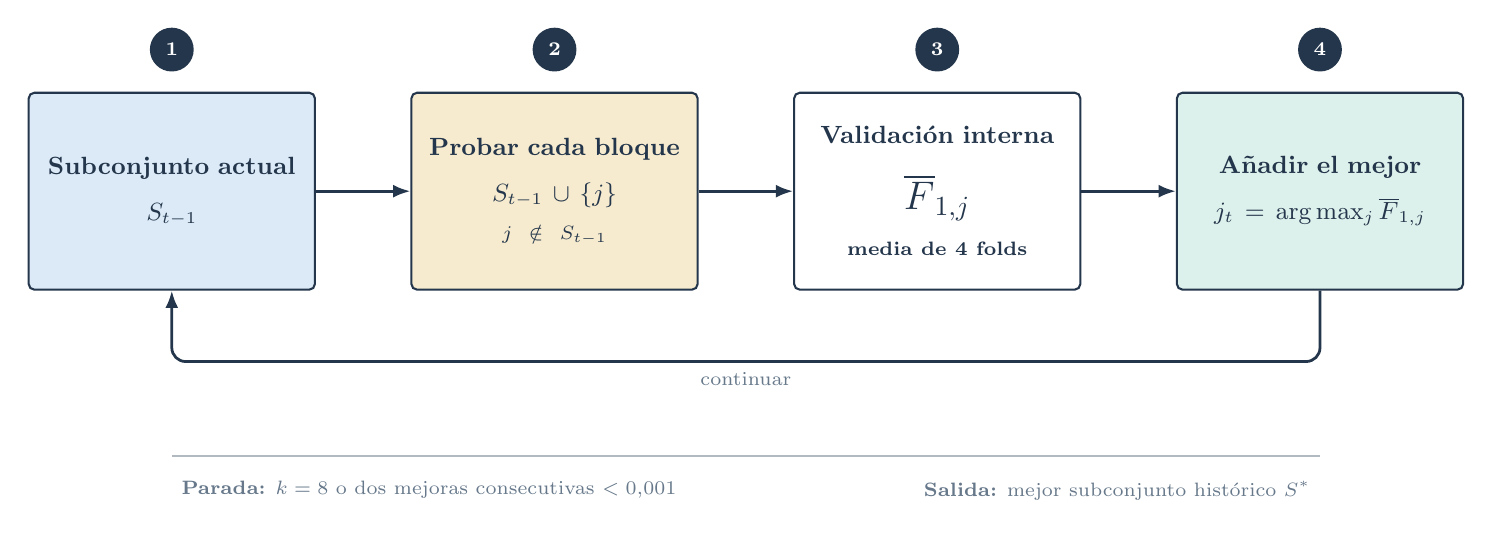
\begin{tikzpicture}[font=\small,node distance=12mm]
  \node[gfsstage,fill=blue] (current) {\bfseries Subconjunto actual\\[2mm]$S_{t-1}$};
  \node[gfsstage,fill=amber,right=of current] (candidates) {\bfseries Probar cada bloque\\[2mm]$S_{t-1}\cup\{j\}$\\[1mm]\scriptsize $j\notin S_{t-1}$};
  \node[gfsstage,fill=white,right=of candidates] (validate) {\bfseries Validación interna\\[2mm]\Large $\overline{F}_{1,j}$\\[2mm]\scriptsize media de 4 folds};
  \node[gfsstage,fill=teal,right=of validate] (choose) {\bfseries Añadir el mejor\\[2mm]$j_t=\arg\max_j\overline{F}_{1,j}$};

  \foreach \n/\x in {1/current,2/candidates,3/validate,4/choose}
    \node[badge,above=2.5mm of \x] {\n};
  \draw[flow] (current) -- (candidates);
  \draw[flow] (candidates) -- (validate);
  \draw[flow] (validate) -- (choose);
  \draw[flow,rounded corners=5pt] (choose.south) -- ++(0,-9mm) -| node[pos=.25,below,note]{continuar} (current.south);

  \coordinate (rulebase) at ($(candidates.south)!0.5!(validate.south)+(0,-18mm)$);
  \draw[ink!35,line width=.6pt] ($(current.south)+(0,-21mm)$) -- ($(choose.south)+(0,-21mm)$);
  \node[note,anchor=north west] at ($(current.south)+(0,-23mm)$)
    {\textbf{Parada:} $k=8$ o dos mejoras consecutivas $<0{,}001$};
  \node[note,anchor=north east] at ($(choose.south)+(0,-23mm)$)
    {\textbf{Salida:} mejor subconjunto histórico $S^*$};
\end{tikzpicture}
\end{document}
